%%%%%%%%%%%%%%%%%%%%%%%%%%%%%%%%%%%%%%%%%%%%%%%%%%%%%%%%%%%%%%%%%%%%%%%%%
%
% Presentation template for Scientific Computing seminar
%
%%%%%%%%%%%%%%%%%%%%%%%%%%%%%%%%%%%%%%%%%%%%%%%%%%%%%%%%%%%%%%%%%%%%%%%%%

\documentclass[hyperref={bookmarks=false},11pt,dvipsnames]{beamer}
\usepackage{tabularx}
\usepackage[linesnumbered,ruled,vlined]{algorithm2e}
\usepackage{hyperref}
\setbeamercolor{url}{fg=red}

%%%%%%%%%%%%%%%%%%%%%%%%%%%%%%%%%%%%%%%%%%%%%%%%%%%%%%%%%%%%%%%%%%%%%%%%%
% Course metadata
\newcommand{\coursename}{Bachelor-Seminar \glqq{}Top 10 Algorithms in Data Mining\grqq{}}
\newcommand{\coursenamefootline}{Bachelor-Seminar \glqq{}Top 10 Algorithms in Data Mining\grqq{}}

% In seminars, the presenter of a talk is typically different from the lecturer responsible for the course.
% The following commands allow to have this distinction. The lecturer's name is printed in the banner on the 
% titlepage (if activated) and the presenter's name is passed into the \author{} command.
\newcommand{\presentername}{Marius Graf}
\newcommand{\presenternameshort}{M. Graf}
\newcommand{\lecturername}{Dr.~Marcel Schweitzer}

\author[\presenternameshort]{\presentername}
\institute{Bergische Universität Wuppertal}
\def\englishlanguage{0}             % set to 1 to switch from German to English

%%%%%%%%%%%%%%%%%%%%%%%%%%%%%%%%%%%%%%%%%%%%%%%%%%%%%%%%%%%%%%%%%%%%%%%%%
% Switches for title page design
\def\printbanner{1}                 % set to 1 to print title page banner
\def\printauthor{1}                 % set to 1 if author name should also be printed outside of title banner
\def\printdate{1}                   % set to 1 in order to print date
\def\printinstitute{0} 		          % set to 1 in order to print institute
\def\printcoursename{1}		          % set to 1 to print course name above title and in footline

%%%%%%%%%%%%%%%%%%%%%%%%%%%%%%%%%%%%%%%%%%%%%%%%%%%%%%%%%%%%%%%%%%%%%%%%%
% Other layout switches
\def\coveredtransparent{1}          % set to 1 to make covered items completely invisible
\def\printnavigationsymbols{0}      % set to 1 to activate navigation symbols
\def\printtocatbeginofsection{1}    % print outline slide (with highlighted current section) at beginning of each section
\def\printtocatbeginofsubsection{0} % print outline slide (with highlighted current subsection) at beginning of each subsection
\def\printlion{1}                   % set to 0 to suppress small "Uni-Loewe" icon in top right corner
\def\printpagenumbers{1}            % set to 0 to suppress page numbers in foot line
\def\longtitle{0}                   % Sometimes, very long titles can break the title page layout. In that case, setting this to 1 might improve things

%%%%%%%%%%%%%%%%%%%%%%%%%%%%%%%%%%%%%%%%%%%%%%%%%%%%%%%%%%%%%%%%%%%%%%%%%
\usetheme{HPC}

% Set language options
\if\englishlanguage0
	\PassOptionsToPackage{german,germankw,onelanguage}{algorithm2e}
	\PassOptionsToPackage{ngerman}{babel}
\else
	\PassOptionsToPackage{english}{babel}
\fi

%%%%%%%%%%%%%%%%%%%%%%%%%%%%%%%%%%%%%%%%%%%%%%%%%%%%%%%%%%%%%%%%%%%%%%%%%
% Include useful packages 
\usepackage[utf8]{inputenc}
\usepackage{amsmath}
\usepackage{framed}
\usepackage[ruled,vlined]{algorithm2e}
\usepackage{amssymb}
\usepackage{array}
\usepackage{caption}
\usepackage{bbding}
\usepackage{bm}
\usepackage{hyperref}
\usepackage{tikz}
\usepackage{times}
\usepackage{ifthen}
\usepackage{pgfplots}
\usepackage{alltt}
\usepackage{transparent}
\usepackage{colortbl}
\usepackage{textcomp}
\usepackage{multirow}
\usepackage{babel}


% increase itemize spacing
\let\realitemize\itemize
\let\endrealitemize\enditemize
\renewenvironment{itemize}{%
	\realitemize\setlength{\parskip}{0pt}\setlength{\itemsep}{.24cm}}
{%
	\endrealitemize%
}

% Switch between transparency and invisibility for covered things
\if\coveredtransparent1
	\setbeamercovered{transparent}
\fi

%%%%%%%%%%%%%%%%%%%%%%%%%%%%%%%%%%%%%%%%%%%%%%%%%%%%%%%%%%%%%%%%%%%%%%%%%
% TikZ initializations, in particular for overlays and externalization

\pgfplotsset{compat=1.12}

\tikzstyle{every picture}+=[remember picture]
\tikzstyle{na} = [baseline=-.5ex, xshift = -0.15cm]
\tikzstyle{na2} = [baseline=-.5ex, xshift = -0.35cm]

\tikzset{
	ncbar angle/.initial=90,
	ncbar/.style={
			to path=(\tikztostart)
			-- ($(\tikztostart)!#1!\pgfkeysvalueof{/tikz/ncbar angle}:(\tikztotarget)$)
			-- ($(\tikztotarget)!($(\tikztostart)!#1!\pgfkeysvalueof{/tikz/ncbar angle}:(\tikztotarget)$)!\pgfkeysvalueof{/tikz/ncbar angle}:(\tikztostart)$)
			-- (\tikztotarget)
		},
	ncbar/.default=0.5cm,
}

\tikzset{square left brace/.style={ncbar=0.5cm}}
\tikzset{square right brace/.style={ncbar=-0.5cm}}

\tikzset{round left paren/.style={ncbar=0.5cm,out=120,in=-120}}
\tikzset{round right paren/.style={ncbar=0.5cm,out=60,in=-60}}
\usetikzlibrary{positioning,matrix,arrows,arrows.meta,backgrounds,shapes}
\usetikzlibrary{backgrounds,mindmap,decorations.pathreplacing,external,calc}
\tikzexternalize[prefix=tikzfigures/] % path for saving precompiled tikz pictures

% Command for easily connecting tikz anchors on slide by arrow
\newcommand{\connectbyarrow}[3]{%
	\begin{tikzpicture}[overlay]
		\path[->,UniGruen,very thick,shorten >= .25cm, shorten <= .25cm] (#1) edge [#3] (#2);
	\end{tikzpicture}
}

%%%%%%%%%%%%%%%%%%%%%%%%%%%%%%%%%%%%%%%%%%%%%%%%%%%%%%%%%%%%%%%%%%%%%%%%%
% Some layout stuff

% set custom text margins
\setbeamersize{text margin left=1em,text margin right=1em}

% Turn off navigation symbols if desired
\if\printnavigationsymbols0
	\beamertemplatenavigationsymbolsempty
\fi

% footline design
\setbeamertemplate{footline}{
	\begin{beamercolorbox}[sep=2pt]{footline}
		\hspace{1em}\insertshortauthor\\ \textit{\insertshorttitle{} \ifthenelse{\printcoursename=1}{(\coursenamefootline)}{}} \hfill
		\ifthenelse{\printpagenumbers=1}{\insertframenumber/\inserttotalframenumber}{} \hspace{1pt}
	\end{beamercolorbox}
}

% custom commands for removing some slides from miniframes (needed for table of contents
% at beginning of section/subsection, see below)
\makeatletter
\let\beamer@writeslidentry@miniframeson=\beamer@writeslidentry
\def\beamer@writeslidentry@miniframesoff{%
	\expandafter\beamer@ifempty\expandafter{\beamer@framestartpage}{}%
	{%
		\clearpage\beamer@notesactions%
	}
}
\newcommand*{\miniframeson}{\let\beamer@writeslidentry=\beamer@writeslidentry@miniframeson}
\newcommand*{\miniframesoff}{\let\beamer@writeslidentry=\beamer@writeslidentry@miniframesoff}
\beamer@compresstrue
\makeatother

% Print table of contents at beginning of each section, with the current section highlighted in green and everything else shaded
\if\printtocatbeginofsection1
	\AtBeginSection[]
	{
		% Remove frame number from footline on outline slides
		\let\rememberpagenumberswitch\printpagenumbers
		\def\printpagenumbers{0}
		\miniframesoff
		\begin{frame}[t,noframenumbering]{\ifthenelse{\englishlanguage=1}{Outline}{Inhalt}}
			\setbeamercolor{section in toc}{fg=UniGruen,bg=}
			\setbeamercolor{section in toc shaded}{fg=Gray,bg=}
			\setbeamercolor{subsection in toc shaded}{fg=Gray,bg=}
			\setbeamercolor{subsection in toc}{fg=Gray,bg=}
			\tableofcontents[currentsection]
		\end{frame}
		\miniframeson
		\let\printpagenumbers\rememberpagenumberswitch
	}
\fi

% Print table of contents at beginning of each subsection, with the current section and subsection highlighted in green and everything else shaded
\if\printtocatbeginofsubsection1
	\AtBeginSubsection[]
	{
		% Remove frame number from footline on outline slides
		\let\rememberpagenumberswitch\printpagenumbers
		\def\printpagenumbers{0}
		\miniframesoff
		\begin{frame}[t,noframenumbering]{\ifthenelse{\englishlanguage=1}{Outline}{Inhalt}}
			\setbeamercolor{section in toc}{fg=UniGruen,bg=}
			\setbeamercolor{section in toc shaded}{fg=Gray,bg=}
			\setbeamercolor{subsection in toc shaded}{fg=Gray,bg=}
			\setbeamercolor{subsection in toc}{fg=UniGruen,bg=}
			\tableofcontents[currentsection,currentsubsection]
		\end{frame}
		\miniframeson
		\let\printpagenumbers\rememberpagenumberswitch
	}
\fi

% Include small "Uni-Loewe" icon in top right corner of each slide
\if\printlion1
	\addtobeamertemplate{frametitle}{}{%
		\tikzexternaldisable%
		\begin{tikzpicture}[remember picture,overlay]%
			\node[anchor=north east,yshift=1.5pt, xshift = 0.2pt] at (current page.north east) {
\includegraphics[height=.6cm]{figures/loewe-weiss.pdf}};%
		\end{tikzpicture}%
		\tikzexternalenable%

		\vspace{-.5cm}
	}
\fi

%%%%%%%%%%%%%%%%%%%%%%%%%%%%%%%%%%%%%%%%%%%%%%%%%%%%%%%%%%%%%%%%%%%%%%%%%
% Title page

% Do not count title page in page numbering
\let\otp\titlepage
\renewcommand{\titlepage}{\otp\addtocounter{framenumber}{-1}}

% Custom title page layout
\defbeamertemplate*{title page}{customized}
{
	\thispagestyle{empty}

	%\vspace{-.5cm}
	\if\printbanner1
		\hpcbanner
	\fi

	\vspace*{.25cm}
	\begin{center}
		\if\printcoursename1
			\Large\textbf{\coursename}\par
		\fi
		\bigskip
		\hfill
		\begin{beamercolorbox}[rounded=true, center, wd=.8\paperwidth]{mycolor}
			\Large\inserttitle
		\end{beamercolorbox}
		\hfill\hfill

		\bigskip
		\bigskip

		\if\printauthor1
			\normalsize\textbf{\insertauthor}\par
		\fi

		\vspace{.15cm}
		\bigskip
		\if\printinstitute1
			\small\insertinstitute\par
		\fi
		\bigskip
		\if\printdate1
			\normalsize\insertdate\par
		\fi
		\ifx\longtitle\undefined
		\else
			\if\longtitle1
				\vspace{-1cm}
			\else

			\fi
		\fi
	\end{center}
}

% Generate HPC banner for title page, similar to our exercise sheet headers etc.
\newcommand{\hpcbanner}{
	\makebox[\textwidth][c]{
		\begin{tikzpicture}
			[textnode/.style={white,font={\bf \sffamily \small},inner sep=0pt}]
			\fill [UniGruen] (0,0) rectangle (\paperwidth,2cm);
			\node [inner sep=0pt] (loewe) at (1,1) {
\includegraphics[width=1.75cm]{figures/loewe-weiss.pdf}};
			\node [textnode,anchor=west] (T) at (2.25,1) {\ifthenelse{\englishlanguage=1}{Scientific Computing \& High Performance Computing}{Wissenschaftliches Rechnen und Hochleistungsrechnen}};
			\node [textnode,above=0.6cm of T.west,anchor=west] {Bergische Universität Wuppertal};
			\node [textnode,below=0.6cm of T.west,anchor=west] {\lecturername};
		\end{tikzpicture}
	}
}

%%%%%%%%%%%%%%%%%%%%%%%%%%%%%%%%%%%%%%%%%%%%%%%%%%%%%%%%%%%%%%%%%%%%%%%%%
% Auxiliary stuff

% Remove algorithm numbering
\renewcommand{\thealgocf}{}

% Command for including small book icon that can be used for referencing literature, lecture notes or similar
\newcommand{\smallbook}{
\includegraphics[width = .028\textwidth]{figures/bookicon.pdf}}

% Command that generates a framed box containing a book icon and text
\newcommand{\inbook}[1]{{\setlength{\topsep}{0pt}
			\begin{framed}
				\begin{minipage}{.08\textwidth}
					
\includegraphics[width = .99\textwidth]{figures/bookicon.pdf}
				\end{minipage}
				\begin{minipage}{.9\textwidth}
					#1
				\end{minipage}
			\end{framed}}}

% Slight change of bibliography layout to look better on slides
\let\OLDthebibliography\thebibliography
\renewcommand\thebibliography[1]{
	\OLDthebibliography{#1}
	\setlength{\parskip}{0pt}
	\setlength{\itemsep}{0pt plus 0.3ex}
}

%%%%%%%%%%%%%%%%%%%%%%%%%%%%%%%%%%%%%%%%%%%%%%%%%%%%%%%%%%%%%%%%%%%%%%%%%
% Some commands that I frequently need
\newcolumntype{C}[1]{>{\centering\arraybackslash}p{#1}}
% Define your logos here to be used on the title page
\newcommand{\BUWLogo}{
\includegraphics[height=32pt]{figures/loewe-weiss.pdf}}
\newcommand{\upk}{^{(k)}}
\newcommand{\upm}{^{(m)}}
\newcommand{\upinv}{^{-1}}
\newcommand{\R}{\mathbb{R}}
\newcommand{\N}{\mathbb{N}}
\newcommand{\C}{\mathbb{C}}
\newcommand{\K}{\mathcal{K}}
\newcommand{\bigO}{\mathcal{O}}
\newcommand{\Rn}{\mathbb{R}^n}
\newcommand{\Rk}{\mathbb{R}^k}
\newcommand{\Cn}{\mathbb{C}^n}
\newcommand{\Rnn}{\mathbb{R}^{n \times n}}
\newcommand{\Cnn}{\mathbb{C}^{n \times n}}
\newcommand{\slitplane}{\mathbb{C} \setminus \mathbb{R}_0^-}
\newcommand{\va}{{\mathbf a}}
\newcommand{\vb}{{\mathbf b}}
\newcommand{\vc}{{\mathbf c}}
\newcommand{\vd}{{\mathbf d}}
\newcommand{\vdhat}{{\mathbf {\hat d}}}
\newcommand{\ve}{{\mathbf e}}
\newcommand{\vehat}{{\mathbf {\hat e}}}
\newcommand{\vf}{{\mathbf f}}
\newcommand{\vftilde}{{\mathbf {\widetilde f}}}
\newcommand{\vg}{{\mathbf g}}
\newcommand{\vh}{{\mathbf h}}
\newcommand{\vhhat}{{\mathbf {\hat h}}}
\newcommand{\vk}{{\mathbf k}}
\newcommand{\vp}{{\mathbf p}}
\newcommand{\vq}{{\mathbf q}}
\newcommand{\vr}{{\mathbf r}}
\newcommand{\vs}{{\mathbf s}}
\newcommand{\vt}{{\mathbf t}}
\newcommand{\vu}{{\mathbf u}}
\newcommand{\vv}{{\mathbf v}}
\newcommand{\vw}{{\mathbf w}}
\newcommand{\vx}{{\mathbf x}}
\newcommand{\vy}{{\mathbf y}}
\newcommand{\vz}{{\mathbf z}}
\newcommand{\vnull}{\boldsymbol{0}}
\newcommand{\vone}{\boldsymbol{1}}
\newcommand{\spK}{{\cal K}}
\newcommand{\spEK}{{\cal E}}
\newcommand{\spL}{{\cal L}}
\newcommand{\spP}{{\cal P}}
\newcommand{\tol}{\texttt{tol}{}}
\newcommand{\specialcell}[2][l]{\begin{tabular}[#1]{@{}c@{}}#2\end{tabular}}
\renewcommand{\d}{\,\mathrm{d}}
\newcommand{\dmu}{\d\mu(t)}
\newcommand{\dalpha}{\d\alpha(z)}
\DeclareMathOperator{\Pe}{Pe}
\DeclareMathOperator{\spec}{spec}
\DeclareMathOperator{\diag}{diag}
\DeclareMathOperator{\range}{range}
\DeclareMathOperator{\Span}{span}
\DeclareMathOperator{\trace}{trace}
\DeclareMathOperator{\tr}{tr}
\DeclareMathOperator{\sign}{sign}
\DeclareMathOperator*{\argmin}{arg\,min}
\DeclareMathOperator*{\argmax}{arg\,max}
\newcommand{\lmin}{{\lambda_{\min}}}
\newcommand{\lmax}{{\lambda_{\max}}}
\newcommand{\AHA}{A^H\!A}
\newcommand{\tve}{\widetilde{{\mathbf e}}}
\newcommand{\tvf}{\widetilde{{\mathbf f}}}
\newcommand{\tvx}{\widetilde{{\mathbf x}}}
\newcommand{\tvr}{\widetilde{{\mathbf r}}}
\newcommand{\rhoinvA}{\rho}
\newcommand{\deltaA}{\delta}
\newcommand{\deltainvA}{\delta'}
\newcommand{\Lmax}{\Lambda_{\max}}
\newcommand{\nmin}{\nu_{\min}}
\newcommand{\nmax}{\nu_{\max}}
\newcommand{\calO}{\mathcal{O}}
\newcommand{\comment}[1]{{\small\color{gray!50}// #1}}
\DeclareMathAlphabet{\mathbf}{OT1}{cmr}{bx}{n}
\def\Hat{\mkern-3mu\text{\textasciicircum}}
 

\title{AdaBoost}
\date{06.12.2023}

\begin{document}

%%%%%%%%%%%%%%%%%%%%%%%%%%%%%%%%%%%%%%%%%%%%%%%%%%%%%%%%%%%%%%%%
% title slide
\maketitle
%%%%%%%%%%%%%%%%%%%%%%%%%%%%%%%%%%%%%%%%%%%%%%%%%%%%%%%%%%%%%%%%


%%%%%%%%%%%%%%%%%%%%%%%%%%%%%%%%%%%%%%%%%%%%%%%%%%%%%%%%%%%%%%%%
% outline slide (without frame number in foot line)
\let\rememberpagenumberswitch\printpagenumbers
\def\printpagenumbers{0}

\begin{frame}[t,noframenumbering]{\ifthenelse{\englishlanguage=1}{Outline}{Inhalt}}
	\tableofcontents
\end{frame}
\let\printpagenumbers\rememberpagenumberswitch
%%%%%%%%%%%%%%%%%%%%%%%%%%%%%%%%%%%%%%%%%%%%%%%%%%%%%%%%%%%%%%%%


%%%%%%%%%%%%%%%%%%%%%%%%%%%%%%%%%%%%%%%%%%%%%%%%%%%%%%%%%%%%%%%%%%%%%%%%%
%
% Content starts here
%
%%%%%%%%%%%%%%%%%%%%%%%%%%%%%%%%%%%%%%%%%%%%%%%%%%%%%%%%%%%%%%%%%%%%%%%%%

\section{Einleitung}

\begin{frame}[t]{Was ist Data Mining?}
	
\includegraphics[width=0.5\textwidth]{figures/datamining.png}
	\begin{itemize}
		\item <1-> Analysiert große Datenmengen, um Muster und Zusammenhänge zu erkennen.
		\item <2-> Nutzt dabei Methoden aus der Statistik, dem Machine Learning und Datenbanktechnologien.
		\item <3-> Spielt eine zentrale Rolle in der Forschung und Industrie,
		      um Erkenntnisse zu gewinnen und
		      Entscheidungen zu unterstützen.
	\end{itemize}
\end{frame}
\begin{frame}[t]{Was sind Ensemble-Methoden?}
	\begin{itemize}
		\item <1-> \textbf{Ensemble-Verfahren:} Kombinieren mehrere Modelle für präzisere Vorhersagen
		\item <2-> \textbf{Fehlerminimierung:} Reduzieren von systematische Fehlern in Modellprognosen
		\item <3-> \textbf{Arten von Ensemble-Methoden:}
		      \begin{itemize}
			      \item Bagging
			      \item Stacking
			      \item Boosting
		      \end{itemize}
		\item <4-> \textbf{AdaBoost gehört zu den Boosting-Verfahren}
	\end{itemize}
\end{frame}

\section{Grundlagen des Boosting}
\begin{frame}[t]{Die Grundidee}
	\begin{itemize}
		\item <2-> Boosting ist eine Ensemble-Methode, die schwache Lerner kombiniert,
		      um ein starkes Gesamtmodell zu bilden.
		\item <3-> Ein schwacher Lerner ist ein Modell, das nur minimal besser als Zufall
		      vorhersagt, indem es schwache Zusammenhänge in den Daten erkennt.
		\item <4-> Durch iterative Anpassung der Gewichtung von Trainingsdaten korrigiert jedes
		      neue Modell die Fehler seiner Vorgänger.
		\item <5-> Das Verfahren zielt darauf ab, den Bias zu verringern und die Vorhersagegenauigkeit
		      für schwer klassifizierbare Beispiele zu erhöhen.
	\end{itemize}
\end{frame}

\begin{frame}[t]{Veranschaulichung}
	\centering
	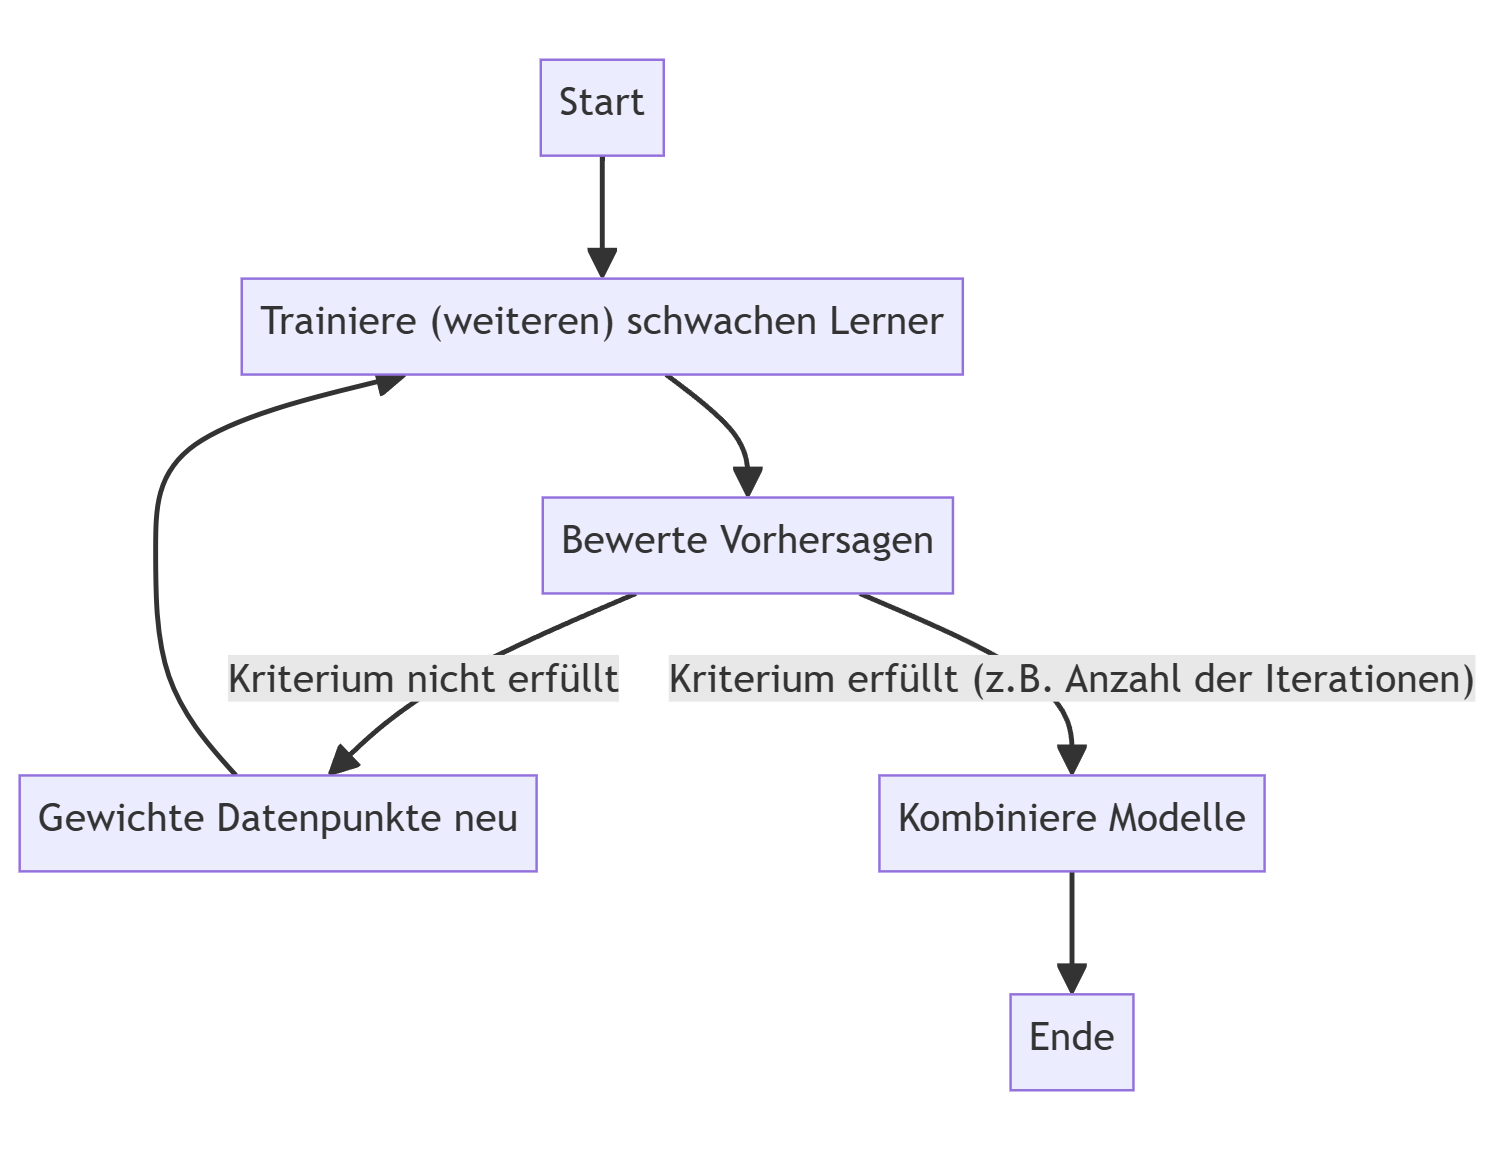
\includegraphics[width=0.8\textwidth]{../Ausarbeitung/figures/Boosting_Graph.png}
\end{frame}
\begin{frame}[t]{Beispiel}{Vorhersage von Hauspreisen}
	\begin{itemize}
		\item <1-> Wir möchten ein Modell entwickeln, das den Preis von
		      Häusern basierend auf verschiedenen Merkmalen wie Größe, Lage, Anzahl der
		      Zimmer und Baujahr vorhersagt.
	\end{itemize}
	\begin{table}
		\centering
		\resizebox{\textwidth}{!}{%
			\begin{tabularx}{\textwidth}{|X|X|X|X|}
    \hline
    \textbf{Haus} & \textbf{Größe $[m^2]$} & \textbf{Lage} & \textbf{Preis} \\
    \hline
    Haus 1        & 100                    & Zentrum       & 500.000€       \\
    \hline
    Haus 2        & 150                    & Vorort        & 300.000€       \\
    \hline
    Haus 3        & 80                     & Zentrum       & 400.000€       \\
    \hline
    Haus 4        & 120                    & Ländlich      & 200.000€       \\
    \hline
\end{tabularx}
		}
		\caption{Beispielhafte Daten für Hauspreise basierend auf Größe und Lage}
	\end{table}


\end{frame}
\subsection*{Beispiel}
\begin{frame}[t]{Beispiel}{Vorhersage von Hauspreisen}
	\begin{itemize}
		\item <1-> Zunächst wählen wir ein sehr einfaches Modell (schwacher Lerner),
		      das den Preis nur anhand der Größe des Hauses vorhersagt.
		\item <2-> In Wirklichkeit variieren die Hauspreise jedoch nicht nur aufgrund
		      ihrer Größe, sondern auch aufgrund anderer Faktoren.
		      Gegend.
		\item <3-> Da unser Modell nur die Größe berücksichtigt und alle anderen Faktoren ignoriert,
		      wird es systematisch den Preis von Häusern in begehrten Lagen unterschätzen und den Preis
		      von Häusern in weniger beliebten Gegenden überschätzen. Dieser systematische Fehler in den
		      Vorhersagen ist der \textbf{Bias}.
	\end{itemize}
\end{frame}

\begin{frame}[t]{Beispiel}{Vorhersage von Hauspreisen}
	\begin{itemize}
		\item Beim Boosting wird das Gewicht von Datenpunkten iterativ so angepasst, dass sich
		      nachfolgende Modelle verstärkt auf zuvor schlecht vorhergesagte Fälle konzentrieren.
	\end{itemize}
	\begin{table}
		\centering
		\resizebox{\textwidth}{!}{%
			\begin{tabularx}{\textwidth}{|X|X|X|X|X|X|}
    \hline
    \textbf{Haus} & \textbf{Größe $[m^2]$} & \textbf{Lage} & \textbf{Preis} & \textbf{Vorhersage (It. 1)} & \textbf{Vorhersage (It. 2)} \\
    \hline
    Haus 1        & 100                    & Zentrum       & 500.000€       & 450.000€                    & 490.000€                    \\
    \hline
    Haus 2        & 150                    & Vorort        & 300.000€       & 350.000€                    & 310.000€                    \\
    \hline
    Haus 3        & 80                     & Zentrum       & 400.000€       & 380.000€                    & 405.000€                    \\
    \hline
    Haus 4        & 120                    & Ländlich      & 200.000€       & 250.000€                    & 210.000€                    \\
    \hline
\end{tabularx}
		}
		\caption{Beispielhafte Daten für Hauspreise und wie Boosting den Bias in mehreren Iterationen reduziert}
	\end{table}
\end{frame}

\section{Der AdaBoost Algorithmus}
\begin{frame}[t]{Einführung}
	\begin{itemize}
		\item <1-> \glqq Adaptive Boosting\grqq
		\item <2-> AdaBoost, entwickelt in den 1990ern von Freund und Schapire, ist ein
		      einflussreiches Verfahren für binäre Klassifikation im maschinellen Lernen.
		\item <3-> Es nutzt eine iterative Boosting-Methode, die die Gewichtung falsch
		      klassifizierter Datenpunkte erhöht, um die Vorhersagegenauigkeit zu verbessern.
		\item <4-> AdaBoosts spezielle adaptive Fehlerkorrektur hebt es von anderen Boosting-Methoden ab und hat zu
		      vielen Weiterentwicklungen geführt.
	\end{itemize}\cite{WuKumar2009}
\end{frame}

\begin{frame}{Vereinfachte Sicht auf den Algorithmus}
	\begin{algorithm}[H]
		\DontPrintSemicolon
		\SetKwInput{KwData}{Daten}
		\SetKwInput{KwResult}{Ergebnis}
		\BlankLine
		\KwIn{Datensatz, Lernalgorithmus}
		Initialisiere Gewichte des Datensatzes\;
		\For{\(t = 1\) \KwTo \(T\)}{
			Trainiere schwache Lerner mit gewichtetem Datensatz\;
			Bestimme Fehler der Lerner\;
			Wähle schwachen Lerner mit geringstem Fehler\;
			Berechne Lernkoeffizienten\;
			Gewichte Datenpunkte neu\;
		}
		\KwOut{\text{Starker Lerner (Ensemble)}}
	\end{algorithm}
\end{frame}

\begin{frame}[t]{Notation}
	\begin{itemize}
    \item Sei $\mathcal{X}$ die Menge der Features mit $\left|\mathcal{X}\right| = n$
          (Anzahl der Features) und $\mathcal{Y}$ die Menge der Labels, die gelernt werden sollen.
          Dabei ist $\mathcal{Y}=\{-1, +1\}$ bei binärer Klassifikation. Ein Trainingdatensatz $D$ besteht aus $m$ Einträgen,
          welche Features mit Labels verbinden:
          $$
              D=\{(\boldsymbol{x}_i, y_i)\},~i=1, \dots, m
          $$
    \item Nach dem Training auf $D$ wird ein Lernalgorithmus $\mathcal{L}$ eine Hypothese bzw. einen Klassifizierer
          $h$ zurück geben, der von $\mathcal{X}$ nach $\mathcal{Y}$ abbildet.
          \begin{align*}
              h:\mathcal{X} \rightarrow \mathcal{Y}, h(\boldsymbol{x}) = y
          \end{align*}
    \item $T$ ist die Anzahl der gewünschten Trainingsiterationen.
    \item Bei jeder Iteration $t=1, \dots,T$ wird ein Datensatz $\mathcal{D}_t$ von $D$ abgeleitet. Dabei wird
          jeder Datenpunkt mit einem Gewicht $\mathcal{D}_t(i)$ mit $i=1, \dots, m$ erweitert.
\end{itemize}

\end{frame}

\begin{frame}[t]{Initialisierung der Gewichte}
	\begin{itemize}
		\item <1-> Zu beginn sind die Gewichte gleich verteilt $$
    \mathcal{D}_1(i) = \frac{1}{m}
$$
		\item <2-> Die Summe der Gewichte ist stets 1 $$
    \sum_{i=1}^m w_i^{(t)}= 1~~\forall t=1,\dots,T
$$
	\end{itemize}
\end{frame}

\begin{frame}[t]{Training der schwachen Lerner}
	\begin{itemize}
		\item <1-> Trainiere für $t=1,\dots,T$ Iterationen schwache Lerner unter berücksichtigung der aktuellen Gewichtung.
$$
    h_t = \mathcal{L}(D, \mathcal{D}_t)
$$
		\item <2-> Das Ziel ist es, den gewichteten Fehler zu minimieren:
$$
    \varepsilon_t = \sum_{i=1}^n {D}_t(i) I\left(y_i \neq h_t\left(\boldsymbol{x}_i\right)\right)
$$ wähle daher den Lerner mit dem geringsten Fehler.
		\item <3-> Indikatorfunktion
$$
    I(A)=\left\{\begin{array}{c c}
        1, & \text{ wenn } A \\
        0, & \text{ sonst}
    \end{array}\right.
$$
	\end{itemize}

\end{frame}

\begin{frame}[t]{Berechnung des Lernkoeffizienten}
	\begin{itemize}
		\item <1-> Zu dem ausgewählten Lerner $h_t$ wird nun ein \textbf{Lernkoeffizient} $\alpha_t$ berechnet:
		      $$
    \alpha_t = \frac{1}{2}\ln\left(\frac{1-\varepsilon_t}{\varepsilon_t}\right)
$$
		\item <2-> Dieser gibt an, wie stark die Vorhersage dieses Lerners im späteren Ensemble gewichtet wird.
	\end{itemize}
\end{frame}

\begin{frame}[t]{Aktualisierung der Gewichte}
	\begin{itemize}
		\item <1-> Die neuen Gewichte der Daten für den nächsten Durchlauf werden berechnet durch
		      \begin{align*}
    \mathcal{D}_{t+1}(i) = & \mathcal{D}_{t}(i) \times e^{-\alpha_t} & \text{ für korrekt klassifizierte Datenpunke} \\
    \mathcal{D}_{t+1}(i) = & \mathcal{D}_{t}(i) \times e^{\alpha_t}  & \text{ für falsch klassifizierte Datenpunke}
\end{align*}
		\item <2-> Die neuen Gewichte müssen anschließend normalisiert werden, damit ihre Summe wieder 1 ist:
		      \begin{align*}
    Z_t                  & =\sum_{j=1}^n\mathcal{D}_{t+1}(j)~(\text{Normalisierungsfaktor}) \\
    \mathcal{D}_{t+1}(i) & = \frac{\mathcal{D}_{t+1}(i)}{Z_t}
\end{align*}
	\end{itemize}
\end{frame}

\begin{frame}[t]{Das Ergebnis des Algorithmus}
	Der Algorithmus gibt ein Gesamtmodell zurück, welches die Klassifizierung des Datenpunktes durch die gewichtete
Summe aller schwachen Lerner darstellt:
\begin{align*}
    H    & :      \mathcal{X} \rightarrow \{-1, +1\}      \\
    H(x) & =  sign\left(\sum_{t=1}^T\alpha_th_t(x)\right)
\end{align*}
\end{frame}

\begin{frame}[allowframebreaks]{Der vollständige Algorithmus}
	\begin{scriptsize}
		\begin{algorithm}[H]
    \DontPrintSemicolon
    \LinesNotNumbered
    \KwData{Trainingsdatensatz \(D\), Anzahl der Iterationen \(T\).}
    \KwResult{Finale Klassifikationsfunktion: \(H(x) = \text{sign}\left(\sum_{t=1}^{T} \alpha_t h_t(x)\right)\).}
    \BlankLine
    \tcp{Initialisiere Gewichte}
    \(w^{(1)}_i=\frac{1}{m}\)\;
    \For{\(t = 1\) \KwTo \(T\)}{
        \tcp{Trainiere schwache Lerner}
        \((h_{j})_{j\in\mathcal{I}} \leftarrow \mathcal{L}(D, w^{(t)}_i)\) \;
        \tcp{Berechne Fehler}
        \For{$j=1$ \KwTo $n$ }{
            \(\varepsilon_j = \sum_{i=1}^{m} w^{(t)}_i\cdot I(y_i \neq h_j(x_i))\)\;
        }
        Wähle Lerner $h_j$ mit minimalem Fehler $\varepsilon_j$ als \(h_t\)\;
        \tcp{Berechne den Lernerkoeffizienten}
        \(\alpha_t = \frac{1}{2} \ln \left( \frac{1 - \varepsilon_t}{\varepsilon_t} \right)\)\;
        % End of Part 1, save last line number if needed
        \tcp{Algorithmus wird fortgesetzt...}
    }
\end{algorithm}
		\begin{algorithm}[H]
    \LinesNotNumbered
    \DontPrintSemicolon
    \SetKwInput{KwData}{Daten}
    \SetKwInput{KwResult}{Ergebnis}
    \BlankLine
    \tcp{Fortsetzung des Algorithmus}
    \tcp{Weiterhin innerhalb des For-Loops}
    \tcp{Aktualisiere die Gewichte für die nächsten Iterationen}
    \eIf{\(y_i = h_t(x_i)\)}{
        \(w^{(t+1)}_i \leftarrow w^{(t)}_i \cdot e^{-\alpha_t}\)\;
    }{
        \(w^{(t+1)}_i \leftarrow w^{(t)}_i \cdot e^{\alpha_t}\)\;
    }
    \tcp{Normalisiere Gewichte}
    \(Z_t \leftarrow \sum_{j=1}^mw^{(t+1)}_i\)\;
    \For{\(i = 1\) \KwTo \(m\)}{
        \(w^{(t+1)}_i \leftarrow \frac{w^{(t+1)}_i}{Z_t}\)\;
    }
    \KwOut{\(H(x)=\text{sign}\left(\sum_{t=1}^T\alpha_th_t(x)\right)\)}
    \tcp{Ende des Algorithmus}
\end{algorithm}
	\end{scriptsize}
\end{frame}

\begin{frame}{Beispiel und Illustration}{Das XOR-Problem}
	\begin{scriptsize}
		$$
    \left\{
    \begin{array}{c}
        (x_1 =(0, +1), y_1=+1) \\
        (x_2 =(0, -1), y_2=+1) \\
        (x_3 =(+1, 0), y_3=-1) \\
        (x_4 =(-1, 0), y_4=-1)
    \end{array}
    \right\}
$$
		\begin{align*}
    h_1(x)=\left\{\begin{array}{r c}
                      +1, & \text{ wenn } (x_1 > -0.5) \\
                      -1, & \text{sonst}
                  \end{array}\right. &
    h_2(x)=\left\{\begin{array}{r c}
                      -1, & \text{ wenn } (x_1 > -0.5) \\
                      +1, & \text{sonst}
                  \end{array}\right. \\[10pt]
    h_3(x)=\left\{\begin{array}{r c}
                      +1, & \text{ wenn } (x_1 > +0.5) \\
                      -1, & \text{sonst}
                  \end{array}\right. &
    h_4(x)=\left\{\begin{array}{r c}
                      -1, & \text{ wenn } (x_1 > +0.5) \\
                      +1, & \text{sonst}
                  \end{array}\right. \\[10pt]
    h_5(x)=\left\{\begin{array}{r c}
                      +1, & \text{ wenn } (x_2 > -0.5) \\
                      -1, & \text{sonst}
                  \end{array}\right. &
    h_6(x)=\left\{\begin{array}{r c}
                      -1, & \text{ wenn } (x_2 > -0.5) \\
                      +1, & \text{sonst}
                  \end{array}\right. \\[10pt]
    h_7(x)=\left\{\begin{array}{r c}
                      +1, & \text{ wenn } (x_2 > +0.5) \\
                      -1, & \text{sonst}
                  \end{array}\right. &
    h_8(x)=\left\{\begin{array}{r c}
                      -1, & \text{ wenn } (x_2 > +0.5) \\
                      +1, & \text{sonst}
                  \end{array}\right. \\[10pt]
\end{align*}
	\end{scriptsize}
\end{frame}

\begin{frame}{Das XOR-Problem}
	\centering
	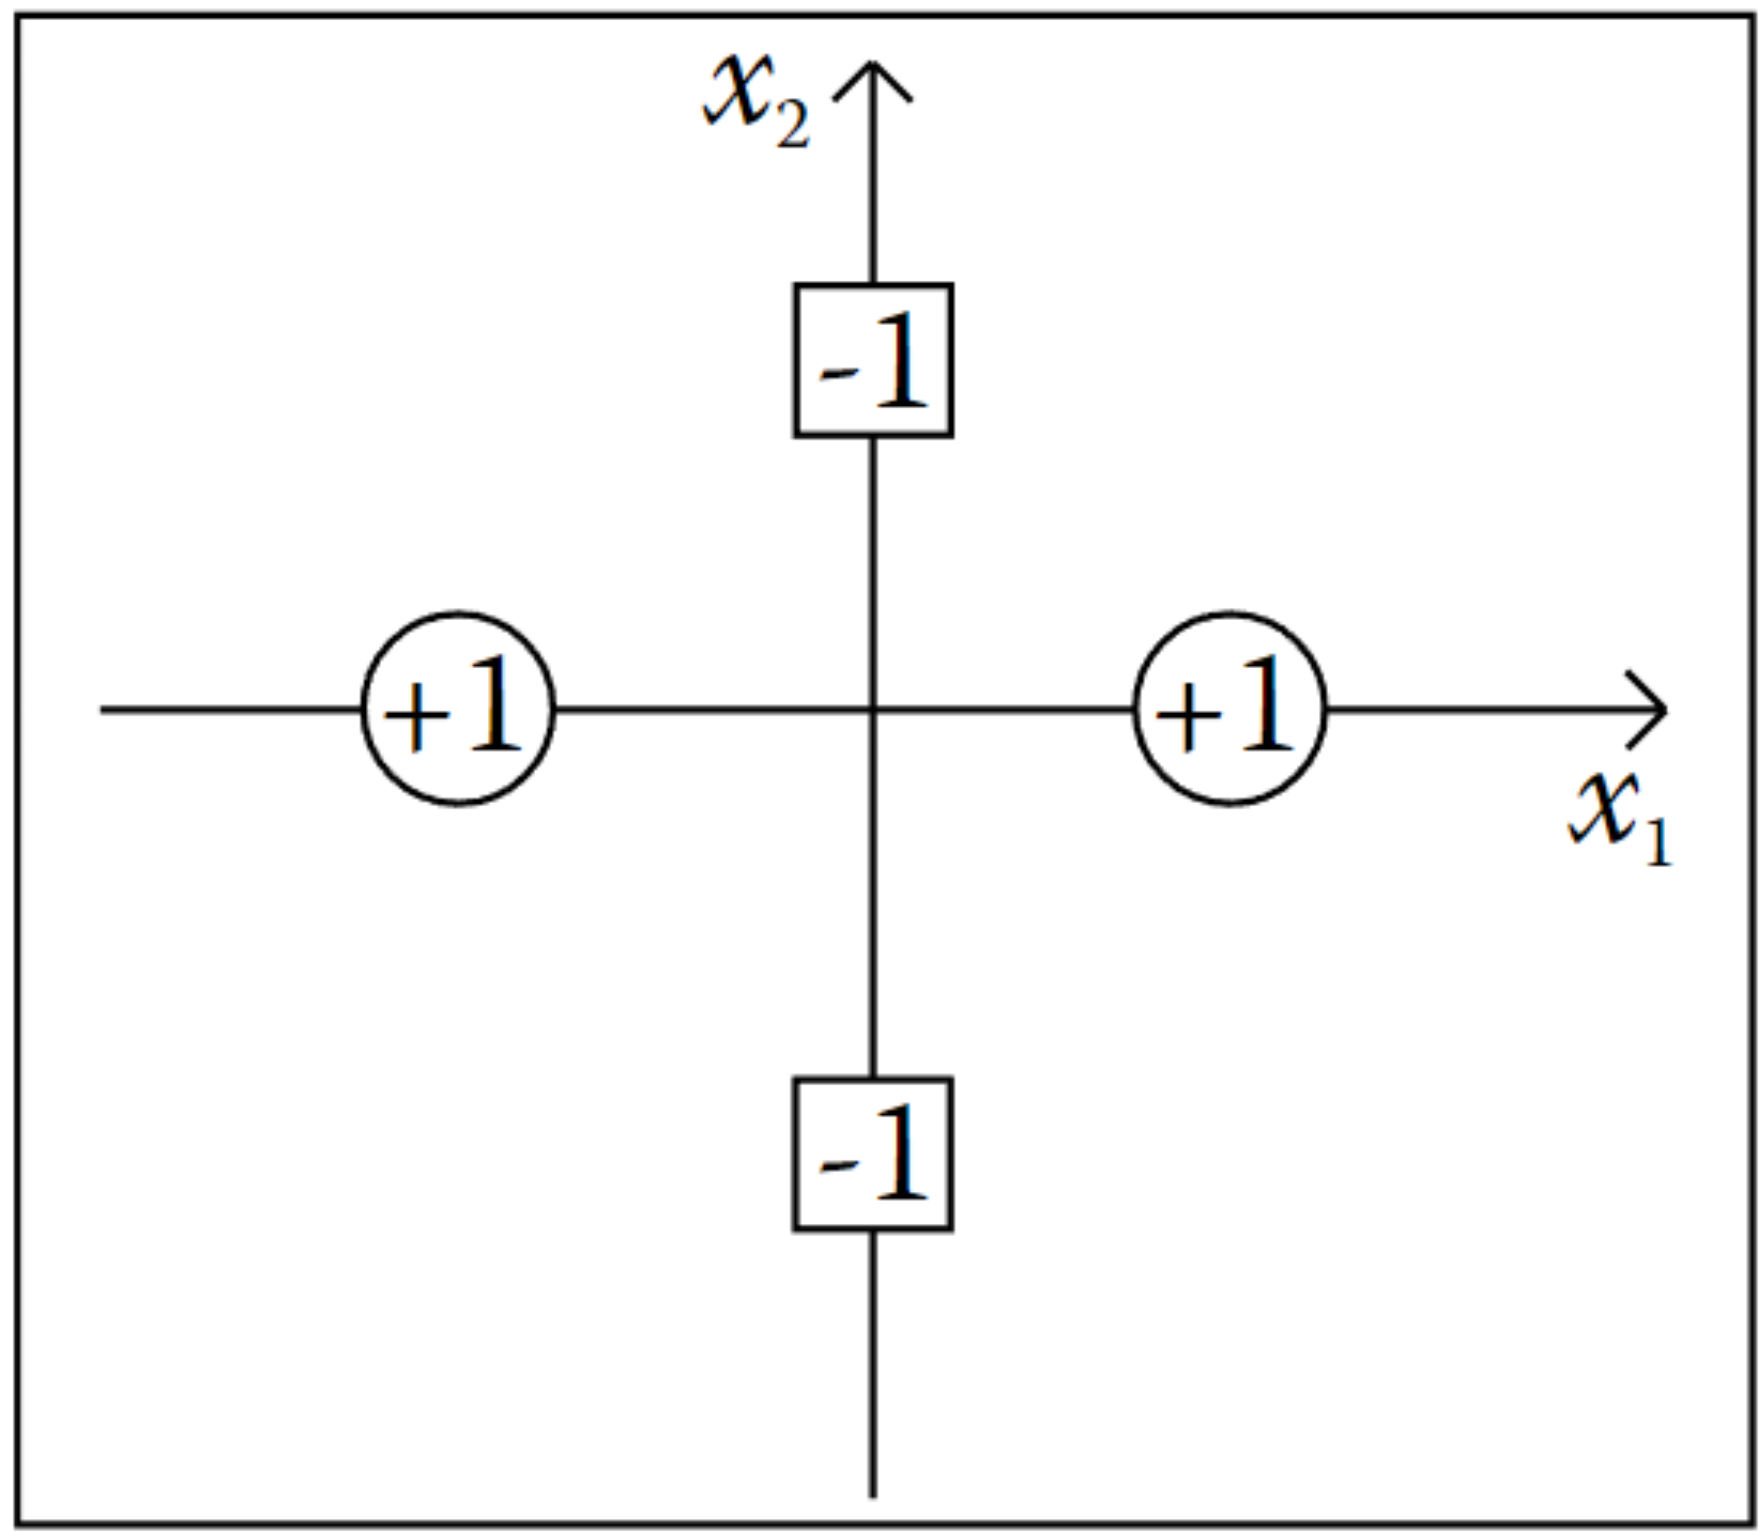
\includegraphics[width=0.5\textwidth]{../Ausarbeitung/figures/XOR-Problem.png}
\end{frame}

\begin{frame}{Das XOR-Problem}
	\centering
	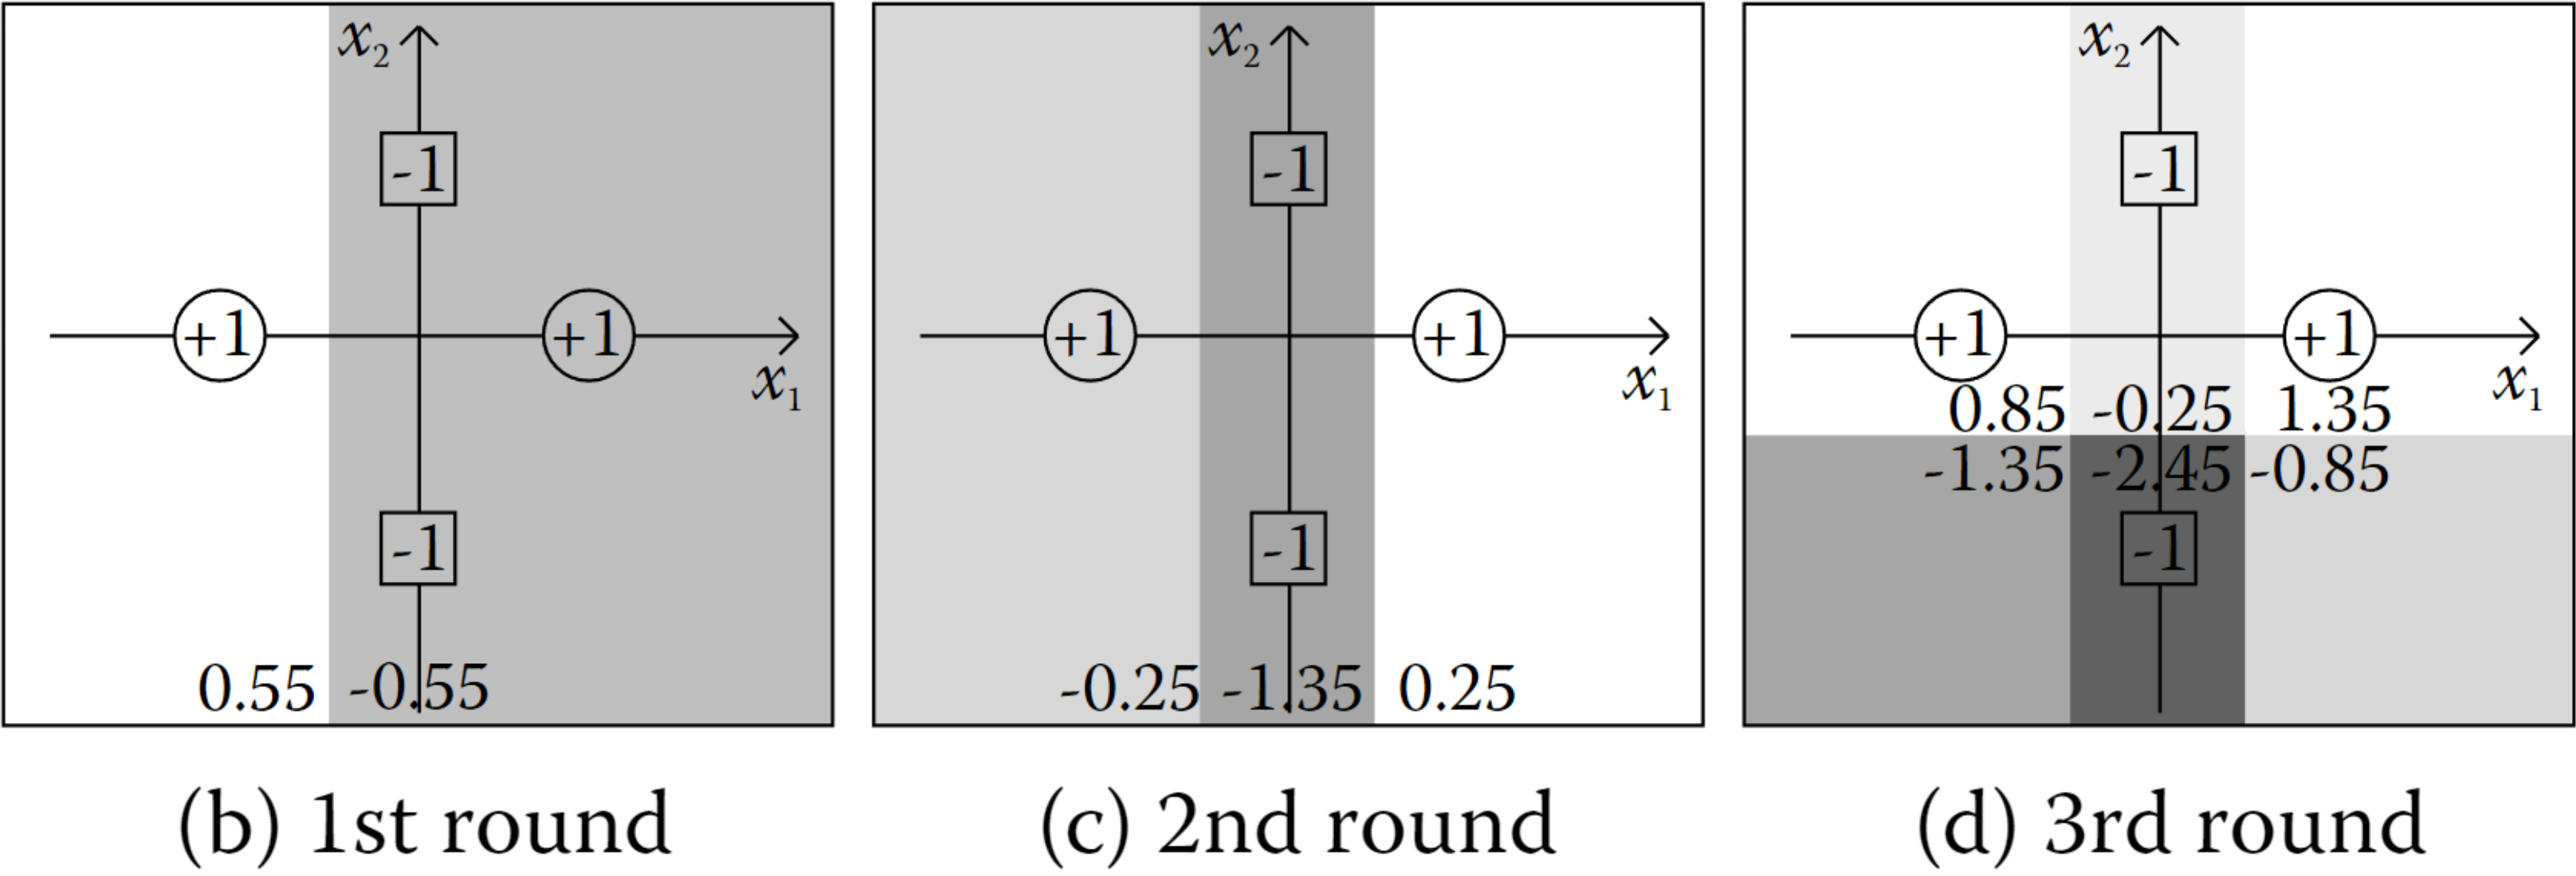
\includegraphics[width=0.8\textwidth]{../Ausarbeitung/figures/XOR_Solution.png}
	\begin{enumerate}
		\item <1-> Basis-Lernalgorithmus wird mit ursprünglichen Daten trainiert; $h_2$
		      wird ausgewählt mit einem Fehler von 0.25 und einem Gewicht von ca. 0.55.
		\item <2-> Nach Erhöhung des Gewichts von $x_1$ wird $h_3$
		      mit einem Fehler von 0.25 und einem Gewicht von 0.80 ausgewählt.
		\item <3-> Gewicht von $x_3$ steigt, $h_5$ wird mit einem Gewicht von
		      1.10 ausgewählt, was zu einem nichtlinearen Klassifikator ohne Fehler führt.
	\end{enumerate}
\end{frame}

\section{Praktische Anwendung}
\begin{frame}{Praktische Anwendung und Beispiele}
	\begin{itemize}
		\item \textbf{Bilderkennung und Computervision:} Gesichtserkennung~\cite{viola2001rapid}
		\item \textbf{Textklassifikation und Natural Language Processing}: Erkennung von Spam-Mail~\cite{panwar2022detection}
		\item \textbf{Medizinische Diagnostik:} Risiko/Erkennung von Krankheiten baserend auf Patientendaten~\cite{hatwell2020ada}
		\item \textbf{Finanzwesen:} Vorhersage von Aktienkursbewegungen~\cite{zhang2016stock}
	\end{itemize}
\end{frame}

\begin{frame}{Praktische Anwendung und Beispiele}
	\begin{figure}
		\centering
		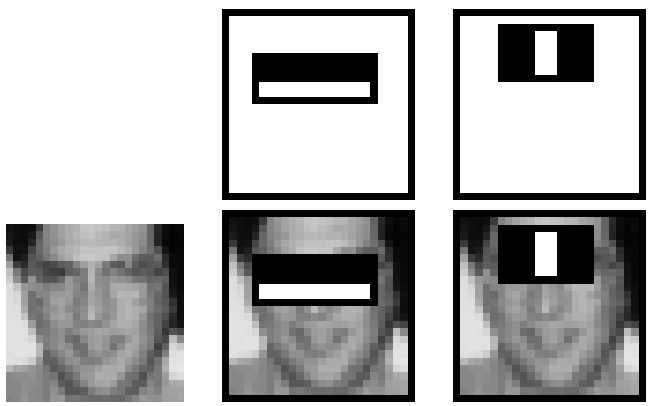
\includegraphics[width=0.5\textwidth]{../Ausarbeitung/figures/CV_Example.png}
		\caption{Anwendung von AdaBoost bei Computer Vision:
			Das erste Merkmal von AdaBoost misst den Intensitätsunterschied
			zwischen der Augenregion und den oberen Wangen,
			wobei die Augen oft dunkler sind. Das zweite Merkmal vergleicht die
			Intensität der Augen mit der Nasenbrücke.\cite{viola2001rapid}}
	\end{figure}
\end{frame}
\section{Vor- und Nachteile}
\begin{frame}{Vor- und Nachteile von AdaBoost}
	\begin{itemize}
		\item <1-> AdaBoost ist benutzerfreundlich, flexibel, und identifiziert
		      automatisch wichtige Features, wobei es weniger zu Overfitting neigt.
		\item <2-> Es ist anfällig für verrauschte Daten und Außreißer, kann bei großen Datensätzen
		      zeitintensiv sein und ist hauptsächlich für binäre Klassifikation ausgelegt.
	\end{itemize}
\end{frame}

\section{Erweiterungen und Variationen}
\begin{frame}{Erweiterungen und Variationen von AdaBoost}
	\begin{itemize}
		\item <1-> ursprünglich für binäre Klassifikation entwickelt,
		      durch verschiedene Erweiterungen für diverse Problemstellungen adaptiert.
		\item <2-> Variationen wie \glqq AdaBoost.M1\grqq~ und \glqq SAMME\grqq~
		      erweitern den Algorithmus für Multiklassen-Probleme.
		\item <3-> Kosten-sensitives AdaBoost passt Gewichtungen basierend auf Fehlerkosten an.
		\item <4-> Neben Entscheidungsstümpfen kann AdaBoost mit SVMs oder
		      Neuronalen Netzen kombiniert werden.

	\end{itemize}
\end{frame}

\begin{frame}{Erweiterungen und Variationen von AdaBoost}
	\begin{itemize}
		\item <1-> Robuste AdaBoost-Varianten minimieren die Auswirkung von Ausreißern.
		\item <2-> Online AdaBoost aktualisiert Modelle mit sequenziellen
		      Daten ohne Neutrainierung.
		\item <3-> Einige Varianten integrieren Feature-Auswahl direkt, um
		      Interpretierbarkeit und Trainingseffizienz zu steigern.
	\end{itemize}
\end{frame}
\section{Literatur und Zusatzmaterial}
\begin{frame}[allowframebreaks]{Literatur}
	\bibliographystyle{alpha}
	\bibliography{../Ausarbeitung/seminar_top10.bib}
\end{frame}
\begin{frame}{Zusatzmaterial}
	\centering
	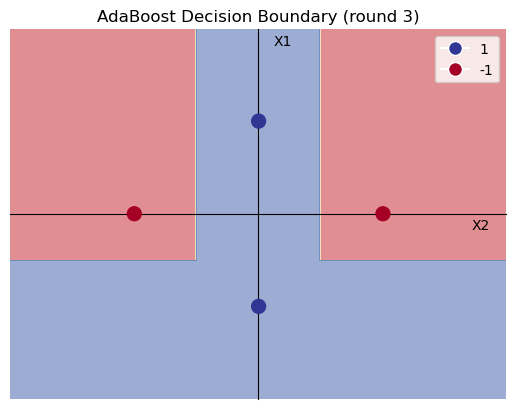
\includegraphics[width=0.45\textwidth]{../Code/img/XOR_Code.png}
	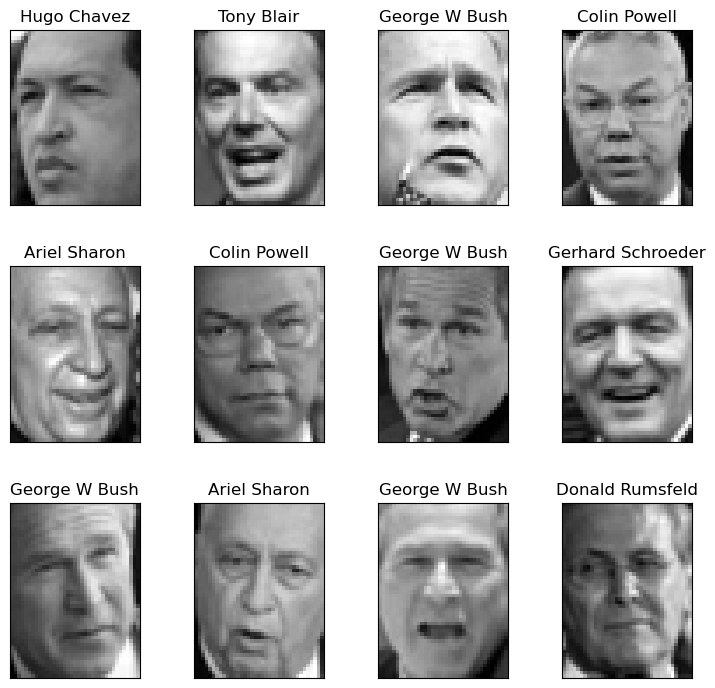
\includegraphics[width=0.45\textwidth]{../Code/img/face_recognition.png}\\
	Umsetzungen und Beispiele von AdaBoost + diese Präsentation mit Ausarbeitung
	in \LaTeX auf \textcolor{red}{\emph{\underline{\href{https://github.com/Vinfeno/TTAIDM_AdaBoost}{GitHub}}}}.
\end{frame}

\begin{frame}{Danke}
	\resizebox{\linewidth}{!}{Vielen Dank für die Aufmerksamkeit!}
\end{frame}
\end{document}



